\documentclass[11pt,a4paper]{article}\usepackage[]{graphicx}\usepackage[]{color}
% maxwidth is the original width if it is less than linewidth
% otherwise use linewidth (to make sure the graphics do not exceed the margin)
\makeatletter
\def\maxwidth{ %
  \ifdim\Gin@nat@width>\linewidth
    \linewidth
  \else
    \Gin@nat@width
  \fi
}
\makeatother

\definecolor{fgcolor}{rgb}{0.345, 0.345, 0.345}
\newcommand{\hlnum}[1]{\textcolor[rgb]{0.686,0.059,0.569}{#1}}%
\newcommand{\hlstr}[1]{\textcolor[rgb]{0.192,0.494,0.8}{#1}}%
\newcommand{\hlcom}[1]{\textcolor[rgb]{0.678,0.584,0.686}{\textit{#1}}}%
\newcommand{\hlopt}[1]{\textcolor[rgb]{0,0,0}{#1}}%
\newcommand{\hlstd}[1]{\textcolor[rgb]{0.345,0.345,0.345}{#1}}%
\newcommand{\hlkwa}[1]{\textcolor[rgb]{0.161,0.373,0.58}{\textbf{#1}}}%
\newcommand{\hlkwb}[1]{\textcolor[rgb]{0.69,0.353,0.396}{#1}}%
\newcommand{\hlkwc}[1]{\textcolor[rgb]{0.333,0.667,0.333}{#1}}%
\newcommand{\hlkwd}[1]{\textcolor[rgb]{0.737,0.353,0.396}{\textbf{#1}}}%
\let\hlipl\hlkwb

\usepackage{framed}
\makeatletter
\newenvironment{kframe}{%
 \def\at@end@of@kframe{}%
 \ifinner\ifhmode%
  \def\at@end@of@kframe{\end{minipage}}%
  \begin{minipage}{\columnwidth}%
 \fi\fi%
 \def\FrameCommand##1{\hskip\@totalleftmargin \hskip-\fboxsep
 \colorbox{shadecolor}{##1}\hskip-\fboxsep
     % There is no \\@totalrightmargin, so:
     \hskip-\linewidth \hskip-\@totalleftmargin \hskip\columnwidth}%
 \MakeFramed {\advance\hsize-\width
   \@totalleftmargin\z@ \linewidth\hsize
   \@setminipage}}%
 {\par\unskip\endMakeFramed%
 \at@end@of@kframe}
\makeatother

\definecolor{shadecolor}{rgb}{.97, .97, .97}
\definecolor{messagecolor}{rgb}{0, 0, 0}
\definecolor{warningcolor}{rgb}{1, 0, 1}
\definecolor{errorcolor}{rgb}{1, 0, 0}
\newenvironment{knitrout}{}{} % an empty environment to be redefined in TeX

\usepackage{alltt}
\usepackage[top=1.00in, bottom=1.0in, left=1.1in, right=1.1in]{geometry}
\usepackage{graphicx}
\usepackage{natbib}
\bibliographystyle{..//..//bib/styles/gcb}
\usepackage{Sweave}

\usepackage[hyphens]{url}
\usepackage[small]{caption}

\setlength\parindent{0pt}

\usepackage{xr}
\usepackage{xr-hyper}

\externaldocument{..//supp/regrisk_supp}
\externaldocument{..//ms/regrisk_submission}

% line numbers for letter
\usepackage{lineno}
\newcommand{\R}[1]{\label{#1}\linelabel{#1}}
\newcommand{\lr}[1]{line~\lineref{#1}}
\IfFileExists{upquote.sty}{\usepackage{upquote}}{}
\begin{document}






\textbf {Reviewer 1 -- comments:} \\

\textit{This manuscript addresses the risk of late spring frost damage to the leaves of temperate trees. The authors use long-term leaf-out phenology records of six European tree species to study the environmental factors that affect the severity of late spring freezes and how climate change is altering these patterns. The main finding is that spring temperature and distance to the coast are the main drivers of spring frost risk, but climate warming is currently altering these trends, complicating forecasts of future spring frost damage. In addition, early-leafing species are found to be more prone to spring freezes with warming, whereas no change or a decrease in spring frost risk was found for late-leafing species. The manuscript addresses an interesting, highly relevant question to better understand the consequences of climate change for plant growth.}\\

We thank the reviewer for this positive feedback and for helping us improve the manuscript. Based on this review we have updated the methods and definitions for all of the models. We believe our revised manuscript better addresses our questions and improves our understanding of the effects of climate change on plant growth.\\

\textit{Yet, I have two major concerns with respect to the methodology of the manuscript.
First, the relevant period during which the leaves of trees are susceptible to freezing events is defined as the 12 days before leaf unfolding (BBCH11). This makes no sense to me. I agree with the assumption that young leaves are more susceptible to freeze events than older leaves and the authors correctly state that ``plants are most susceptible to
damage from freezing temperatures between budburst and full leafout''. However, BBCH 11 is NOT full leafout, it is the stage where the first visible leaf stalk is visible, but not on all buds, only on the first opening buds. Plants are definitely still susceptible to frost after that event. In fact, they should even be more vulnerable to frosts after BBCH11 was reached because the number of buds opening will increase drastically only after BBCH11. The next phenophase available in the PEP725 database (BBCH 13) is the stage were 50\% of leaves are unfolded, which means that even at this later stage, 50\% of leaves are not yet unfolded. So, to me the only way of determining whether the results are robust is to use another approach of calculating the relevant freezing period. Spring freezes after BBCH11 should definitely be accounted for.} \\

We appreciate the concern of Reviewer 1 and have overhauled all the models in our paper to address this. We chose BBCH 11 in part because it is, by far, the most reported spring vegetative phase in PEP 725, yielding 755,087 observations for BBCH 11 in comparison to only 12,417 observations for BBCH 13. After receiving this review we attempted to find sites with both BBCH 11 and BBCH 13 in the same site x species x year so we could estimate the days between them, but such data were virtually non-existent. Thus, to address this we now modify our methodology to include the 12 days before BBCH 11 (as we did before) through 12 days after BBCH 11 as the period of risk. We found these model results---using this 24 day window---were similar to models using a longer window with 24 days after BBCH 11 (Figure \ref{fig:spp}), suggesting we have captured the relevant period.\\ 

{\begin{figure} [H]
  -\begin{center}
  -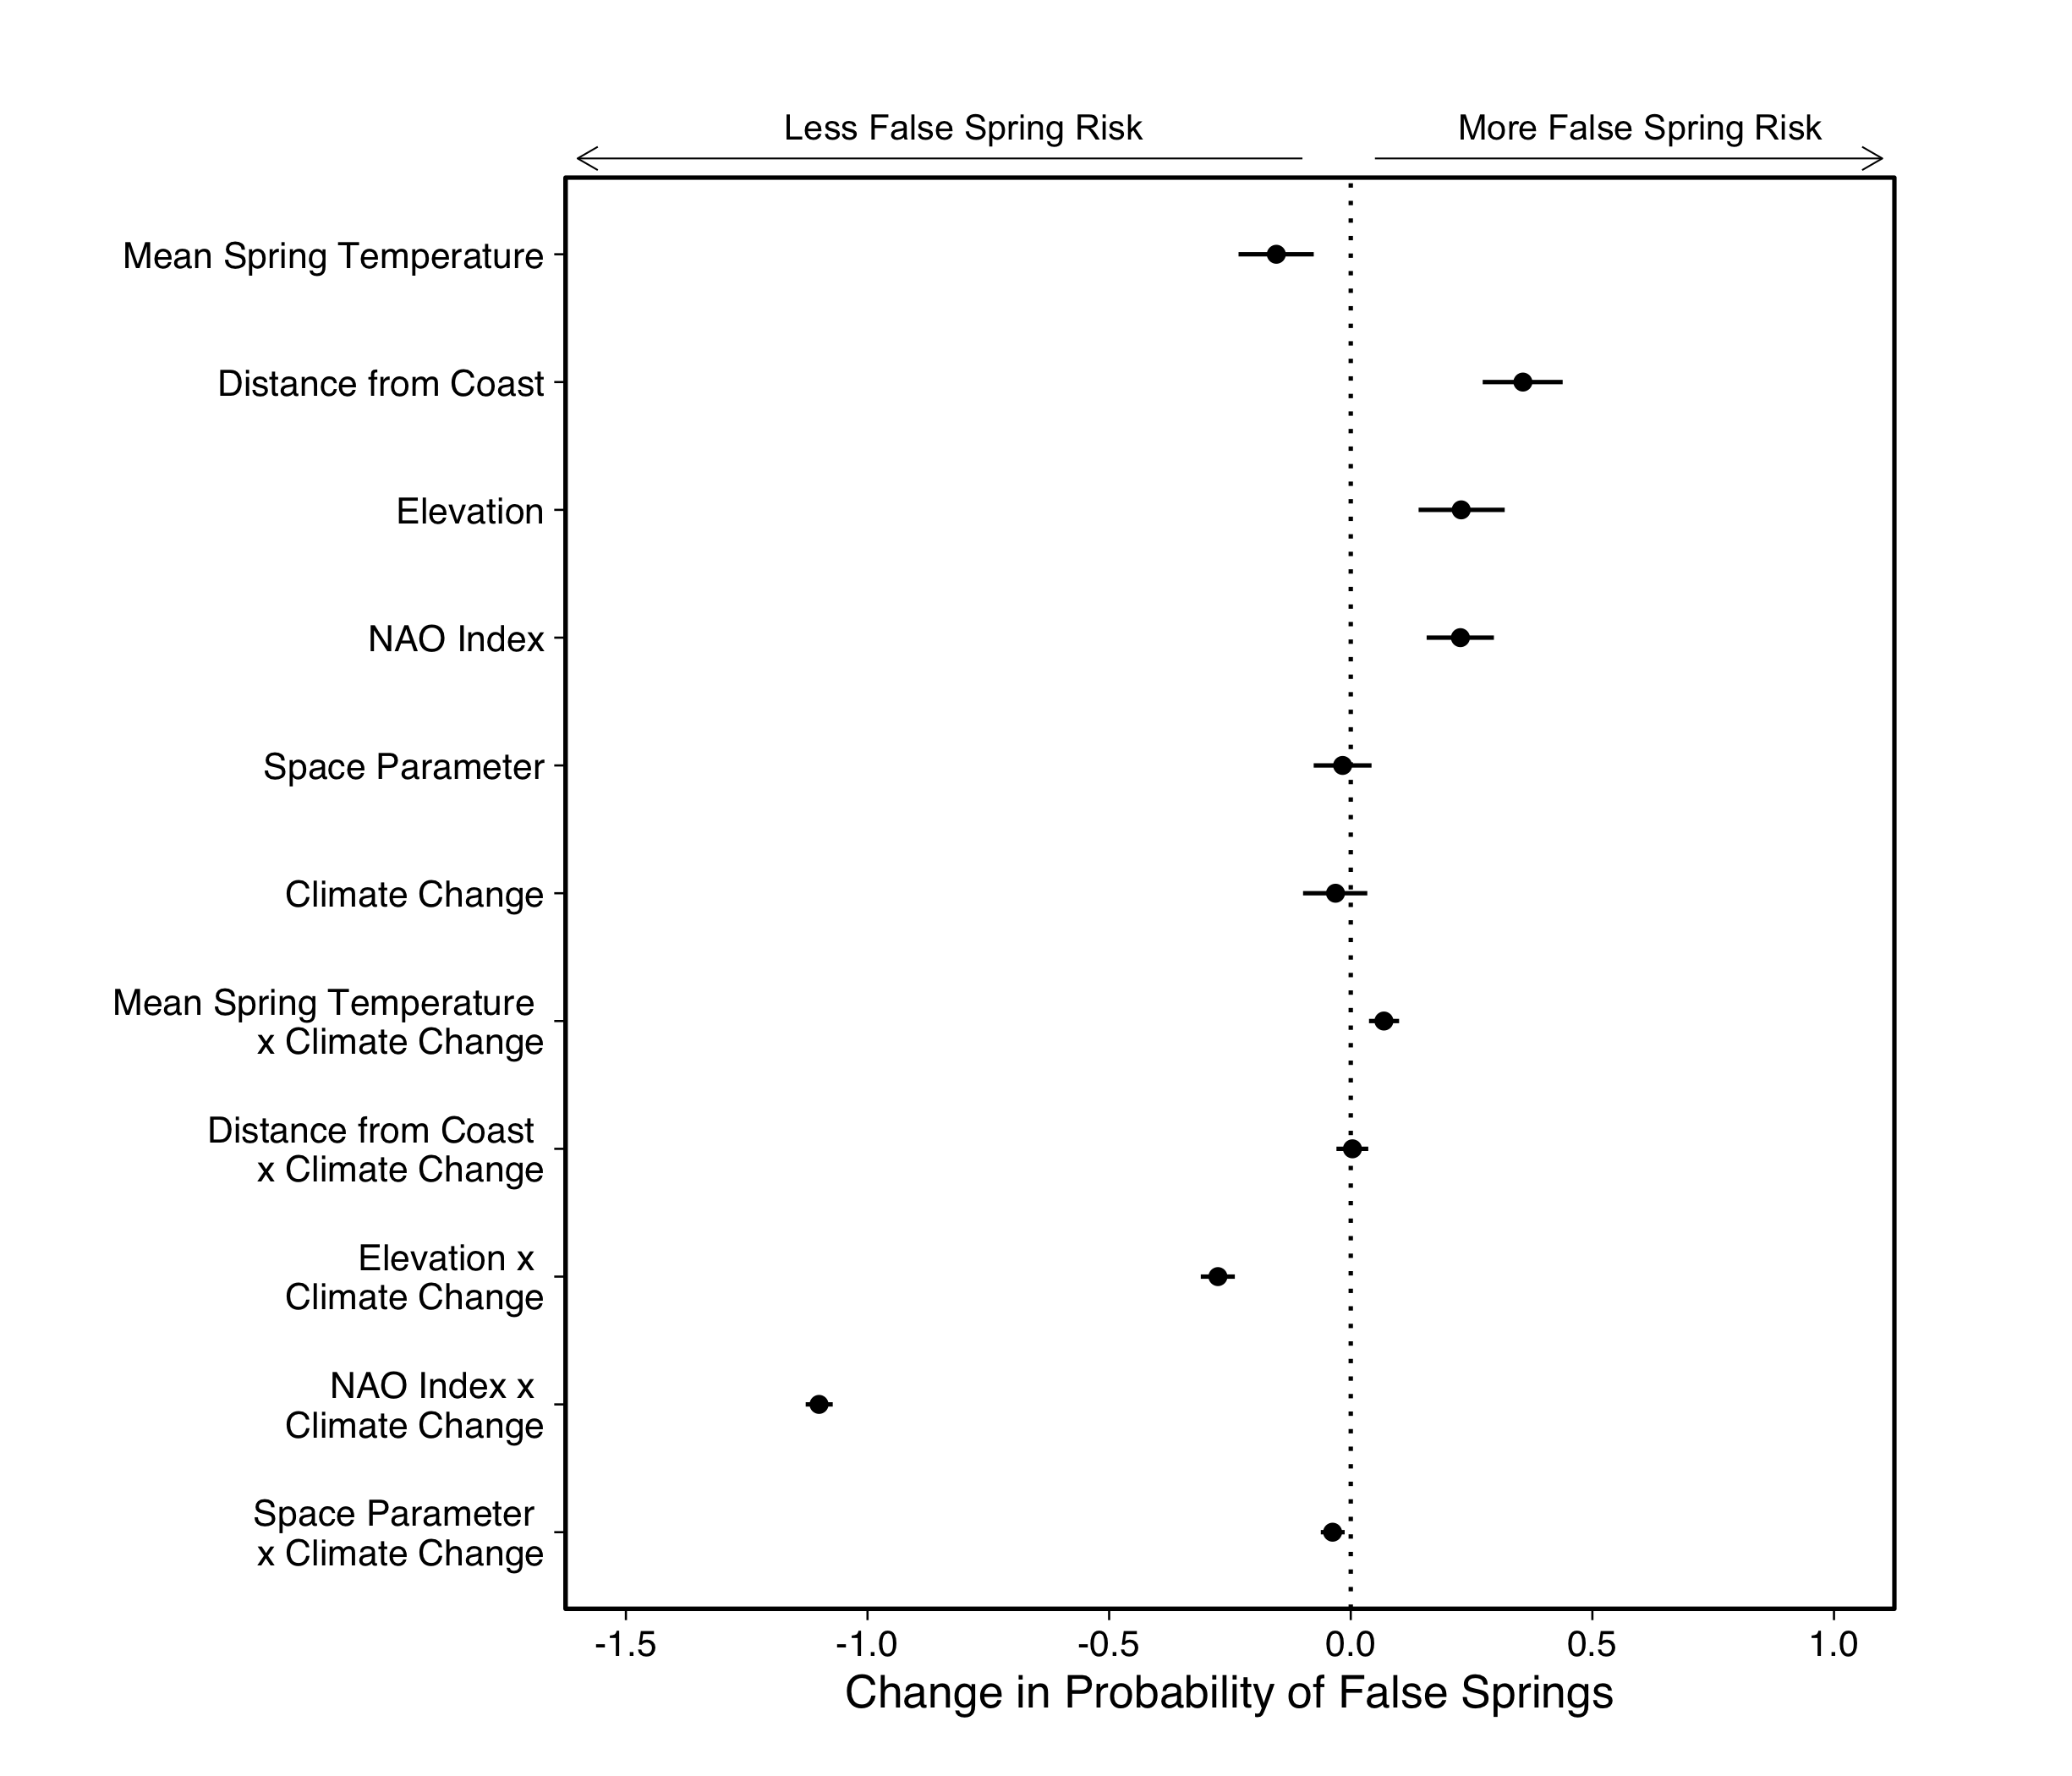
\includegraphics[width=12cm]{..//..//analyses/figures/model_output_98_verylong.png}
  -\caption{Effects of species, climatic and geographical predictors on false spring risk using a 36 day window. More positive values indicate an increased probability of a false spring whereas more negative values suggest a lower probability of a false spring. Dots and lines show means and 98\% uncertainty intervals.}\label{fig:spp}
  -\end{center}
  -\end{figure}}

\newpage
\textit{Second, the study assumes that spring freeze damage will occur at -2.2 C for all species. Yet, leaf-killing temperatures are species-specific (Lenz et al., 2016; Muffler et al., 2016), which should be accounted for when testing for differences among species (Zohner et al., 2020b). Leaves of early-leafing species are usually more freezing resistant than those of late leafers (Muffler et al., 2016). I can see that this problem was partly solved by additionally using -5C as freeze threshold, but this additional analysis only changes the general freezing threshold and still doesn't account for differences among species. The leaves of Aesculus, Alnus, and Betula are more resistant to frost than the leaves of Fagus, Fraxinus, and Quercus (data in Muffler et al., 2016; Zohner et al., 2020a, not yet published but attached to this review). It would therefore be interesting to see whether the species-level results still hold when using a freezing threshold of -2.2 C for the latter group and -5C for the first group of species.} \\

We thank the reviewer for this insight and new idea to improve the manuscript. We have included a new model that uses varying thresholds for early- versus late-leafout species. We have included a new paragraph to the Introduction (\lr{Z1thresh} - \lr{Z1threshend}): 

\begin{quotation}
\noindent Species may vary in their false spring risk for several major reasons. Species that leafout first each spring may be especially at risk of false springs, as their budburst occurs during times of year when the risk of freeze events is relatively high. To date these early-leafout species also appear to advance the most with warming  \citep{Wolkovich2012}. Thus, if climate change increases only the prevalence of late spring freezes, we would expect major increases in false spring risk for these species. In contrast, if climate change has restructured the timing and prevalence of false springs to later in the spring, then later-leafout species may experience major increases in false spring risk with climate change. Additional complexity in these predictions, however, comes from the potential of species-level differences in in their tolerance of low temperatures during leafout \citep{Lenz2013}, and how quickly they progress from budburst to full leafout---when leaf tissue is least resistant to low temperature \citep{Augspurger2009,Lenz2013,Muffler2016,Zohner2020}.
\end{quotation}

Results section \textit{Sensitivity of results to duration of risk and temperature thresholds} (\lr{Z2thresh} - \lr{Z2threshend}): \\

\begin{quotation}
\noindent  Results of climatic and geographic effects, again, remained consistent in our varying threshold model (where we defined a false spring as -5$^{\circ}$C for early-leafout species and -2.2$^{\circ}$C for late-leafout species) with all predictors contributing to risk: mean spring temperature (-10.38\% for every 2$^\circ$ or -0.65 $\pm$ 0.13 probability of risk/standard unit), distance from the coast (2.41\% for every 2$^\circ$C or 0.18 $\pm$ 0.14 probability of risk/standard unit), elevation (7.48\% for every 200m or 0.64 $\pm$ 0.14 probability of risk/standard unit) and NAO (3.74\% for every 2$^\circ$ or 0.28 $\pm$ 0.12 probability of risk/standard unit). There was also a slight increase in false spring risk due to the residual effect of climate change across all six species (29.69\% increase or 1.1832854 $\pm$ 0.06 probability of risk/standard unit; Figure \ref{fig:longtemps} and Table \ref{tab:suppmodlongtemps}). In contrast to our other models, in this model late-leafout species (i.e., \textit{Fagus sylvatica}, \textit{Quercus robur}, \textit{Fraxinus excelsior}) experienced more false springs than the early-leafout species (i.e., \textit{Aesculus hippocastanum}, \textit{Alnus glutinosa}, \textit{Betula pendula}), though after climate change all species experienced a more similar magnitude of risk (Figure \ref{fig:spptemps}). 
\end{quotation}

Discussion section \textit{Variation in risk across species} (\lr{Z3thresh} - \lr{Z3threshend}) to address these results:

\begin{quotation}
\noindent These results, however, hold only for using a common threshold for false spring risk across species. When we applied a model with varying thresholds for early and late species (-5$^{\circ}$C for early-leafout species and -2.2$^{\circ}$C for late-leafout species), we found contrasting results: with late species having the highest overall risk of false springs and climate change making the risks across species more similar. This is in some ways not surprising as this model more than doubles the threshold for a false spring event for early compared to late species thus biasing the model to find such differences, but it highlights the importance of continued research (e.g., \citep{Lenz2013,Muffler2016,Zohner2020}) to estimate the temperature threshold across species, and show species-level findings can be highly dependent on this threshold. In contrast models using species-specific time periods for budburst to leafout or varying the temperature threshold for a false spring event across all species showed similar results to our main model.
\end{quotation}

We have also included new figures and a table in the supplement with model results (Figure S6, S7 and Table S9) and have additionally made changes throughout the Discussion to highlight that the varying threshold model finds that late-leafout species are at a higher risk of false springs but, with warming, species' risk becomes more similar. We believe these results, though tentative, highlight the importance of understanding varying thresholds and how critical it is to the species-level effects we predict with climate change.

\textit{l. 53: reference needed for ``but budburst has advanced roughly twice as fast''. You are saying budburst advanced by, on average, ~5 days per decade. From my own observations it's more like 2-3 days per decade, which would then be similar to the last spring freeze advances.} \\

We thank the reviewer for finding this error and have updated the sentence and have added citations (\lr{Zbbrefbegin} - \lr{Zbbrefend}): \\

\begin{quotation}
\noindent  In Germany, for example, the last freeze date has advanced by 2.6 days per decade since 1955 \citep{Zohner2016}, but budburst has advanced 4.3 days per decade across Central Europe \citep{Fu2014,Vitasse2018}.
\end{quotation}


\textit{l. 360-368: I don't get the point of this discussion on species ranges. The phenological data used here came mostly from Germany and didn't reflect species ranges at all.} \\

We appreciate the reviewer's concern and have updated the language in the Discussion section \textit{Variation in risk across species} (\lr{Z1ranges} - \lr{Z1rangesend}) to provide additional clarity. We hope that this modified section is easier to follow and understand:  \\

\begin{quotation}
\noindent  Though our study focuses on Central Europe, overall habitat preference and range differences among the species could also explain some of the species-specific variation in the results \citep{Chuine2001}, but would require data on more species---and species that vary strongly in their climatic and geographic ranges---for robust analyses. The ranges of the predictors are similar across species within our dataset, but \textit{Betula pendula} extends to the highest elevation and latitude and spans the greatest range of distances from the coast (Figure \ref{fig:bbmap}), while \textit{Quercus robur} experiences the greatest range of mean spring temperatures. Within our species, \textit{Betula pendula} has the largest global distribution, extending the furthest north and east into Asia. The distribution of \textit{Fraxinus excelsior} extends the furthest south (into the northern region of Iran). These global range differences could potentially underlie the unexplained effect of climate change seen in our results and why the climatic and geographic factors failed to explain all of the variation in false spring risk for our species. Future research that captures these spatial, temporal and climatic differences across myriad species could greatly enhance predictions and help us understand these residual effects of climate change. Such research may be particularly useful if it connects how range and habitat differences translate into differences in physiological tolerances and the underlying controllers of budburst and leafout phenology---the factors that proximately shape false spring risk. 
\end{quotation}


\textbf {Reviewer 2 -- comments:} \\


\textit{The authors describe a statistical analysis on the probability of false springs for an extensive set of drivers, in this respect scaling beyond previous studies. The authors conclude that false spring risks are strongly associated with mean spring temperature and distance from coastal waters, with increased risks for early leaf-out species.} \\

\textit{I've appreciated the rather technical write-up, and in particular the future perspectives which were well defined and outline new research avenues. However, I would like to see some things clarified.} \\

We thank the reviewer for this appreciation and for helping us clarify certain sections and improve our figures. Based on this review we have included data availability, updated the methods and definitions for all of the models and enhanced our figures to be more colorblind-friendly.  \\

\textit{First and foremost a practical issue. Given the use of open data, open software I will insist on the open nature of the analysis executed and all source code to be shared. Given PEP725 redistribution rules data can't be distributed, however code to compile the data in the correct data format can. I suggest to use a repository such as github / gitlab / bitbucket to store your code (and revisions) in their native format (i.e. no copied code in txt files, but .R files). All this should ensure reproducibility, transparency and facilitate re-use of code within a research or educational setting.} \\

We completely agree with the reviewer about this concern and apologize for failing to include our data in the first submission. We have included a new section \textit{Data, Code \& Model Output:} (\lr{R2data} - \lr{R2dataend}) with this information. Please note that all raw data are already publicly available at the Pan European Phenology network webpage (PEP725, www.pep725.eu): \\

\begin{quotation}
\noindent  Phenological data is available at the Pan European Phenology network webpage (PEP725, www.pep725.eu). Data and code from the analyses will be available via KNB upon publication and are available to all reviewers upon request. Raw data, {Stan} model code and output are available on github at \url{https://github.com/cchambe12/regionalrisk} and provided upon request.
\end{quotation}

\textit{Furthermore, to what degree do you think the use of leafout instead of budburst influences the analysis? In particular, the data does not take into account delays in development / leafout due to prior false spring damage (e.g. Gu et al. 2008 / Hufkens et al. 2012 / Augspurger 2007). It could therefore be argued that a fixed offset could influence the results. Although acknowledged on lines 272 onward, using the varying offsets, the use of these undamaged developmental responses is a missing confounding factor which should be discussed.} \\

We appreciate the reviewer's concern and this was clearly an important issue as Reviewer 1 also raised it. To address this, we have modified the methodology for all models to include the 12 days before BBCH 11 through 12 days after BBCH 11 as the period of risk, which we hope will capture this possible delay in development due to prior false spring damage. For an extended discussion of this please see our response to Reviewer 1's above (second set of plain font text in response to Reviewer 1).\\

\textit{Also, on line 140 - 145, it is mentioned E-OBS data is used but I see no mention of lapse rate corrections for altitude to correct for site by site differences (e.g. Basler 2016)? Given the absolute temperature thresholds I think this applies.} \\

We thank the reviewer for pointing this out, as it would certainly affect our results if lapse rate corrections were not applied. Our temperature data includes lapse rates for altitude, which we now state, and we have added a citation in Methods section \textit{Climate Data} (\lr{R2clim} - \lr{R2climend}): \\

\begin{quotation}
\noindent  E-OBS version 16 incorporates station altitude in the interpolation scheme, thus spatially explicit information on day-to-day variability in the environmental lapse rate is captured \citep{Cornes2018}.
\end{quotation}


\textit{Finally, some smaller issues: }\\

\textit{I would increase readability of the figures by avoiding pastel colours. Although I'm not colorblind I'm not sure how well this would work for those who are. }\\

\begin{itemize}
\item Use varying line styles instead of colour if possible (Figure 5)
\item  Don't use colours where not needed (Figure 2 and 3 - species labels)
\item  Make sure that points are properly scaled (smaller for Figure 2), or better regrid the data to show spatial trends more consistently
\item Increase the font size on all figures (for axis labels etc)
\end{itemize}

\textit{I think all of these issues are easily addressed, either in discussion (given data limitations) or with the necessary model / driver data adjustments. Good luck, stay safe !} \\

We appreciate the reviewer's concerns about our figures. We reviewed a suite of information about how to restructure our figures for maximum accessibility. We have thus updated the colors using the viridis package in R, which is colorblind-friendly. Additionally, we have removed unnecessary colors, rescaled the points in Figure 2 and increased the font size on all figures.

\newpage
\bibliography{..//..//bib/RegionalRisk.bib}

\end{document}
